% One-pager on Experiment 4 (controlled difference): conclusion first, three findings with their figures.
% Run results/20261024-000548_exp4ctrl; figures from ../exp4/onepager_figures.py; example tokens are the first common row.
% Wording follows the adversarial verification (exp4/LOG.md). Build (from this folder): pdflatex exp4_onepager.tex
\documentclass[10pt]{article}
\usepackage[letterpaper,hmargin=0.5in,vmargin=0.3in]{geometry}
\usepackage[T1]{fontenc}
\usepackage[scaled=0.92]{helvet}
\renewcommand{\familydefault}{\sfdefault}
\usepackage{microtype}
\usepackage{xcolor}
\usepackage{graphicx}
\usepackage{enumitem}
\usepackage[hidelinks]{hyperref}
\setlength{\parindent}{0pt}
\setlength{\parskip}{2pt}
\setlist{nosep,leftmargin=1.2em,itemsep=1.5pt}
\definecolor{cblue}{HTML}{2A78D6}
\definecolor{corange}{HTML}{EB6834}
\definecolor{ink2}{HTML}{52514E}
\definecolor{muted}{HTML}{898781}
\definecolor{axis}{HTML}{C3C2B7}
\definecolor{plane}{HTML}{F4F3EF}
\definecolor{wordbg}{HTML}{DCEAFB}

% token chips: \tb BOS, \tk random filler, \tw inserted word, \tq final token (where attention is measured)
\newcommand{\chip}[3]{{\setlength{\fboxsep}{1pt}\setlength{\fboxrule}{0.4pt}\fcolorbox{#1}{#2}{\strut\ttfamily\footnotesize #3}}\hspace{0.8pt}}
\newcommand{\tb}{\chip{ink2}{ink2}{\color{white}BOS}}
\newcommand{\tk}[1]{\chip{axis}{white}{\color{muted}#1}}
\newcommand{\tw}[1]{\chip{cblue}{wordbg}{#1}}
\newcommand{\tq}[1]{\chip{corange}{white}{\bfseries #1}}
\newcommand{\gap}[1]{{\color{muted}\footnotesize\,\dots\,#1\,\dots\,}}
\newcommand{\ex}[1]{\leavevmode\makebox[1.45cm][l]{\color{ink2}\small\bfseries #1}}
\newcommand{\head}[2]{\par{\large\bfseries #1}\hfill{\color{muted}\footnotesize #2}\\[-3pt]\rule{\linewidth}{0.5pt}\par}

\begin{document}

{\LARGE\bfseries L11H8 is not a previous-token head: it reads nearby countries}\\[3pt]
{\small\color{ink2} GPT-2 small, 200 random rows $\times$ 11 countries per filler type. Each row has two versions that
differ only at position $\tau$. $\Delta$ = attention from the final token $T$ to $\tau$, country $-$ original, per head, at
every distance $T-\tau = 1\ldots31$.}\\[2pt]
\ex{original}\tb\tk{she}\tk{sc}\gap{26 random tokens}\tk{age}\tk{dis}\tq{ious}\hspace{1.2em}%
\ex{country}\tb\tk{she}\tk{sc}\gap{26 random tokens}\tw{France}\tk{dis}\tq{ious}\hspace{0.5em}{\footnotesize\color{muted}($\tau$ = 30, distance 2)}

\vspace{4pt}
\colorbox{plane}{\parbox{\dimexpr\linewidth-2\fboxsep}{\small
\textbf{Conclusion} {\footnotesize\color{muted}(common / rare filler)}
\begin{itemize}
\item \textbf{L11H8 reads countries, and less so the farther away they are.} It gives the previous token only 8\% / 6\% of
  its attention on random text. An adjacent country raises its attention to that spot by \textbf{+0.065 / +0.039}, which is 0.036 more than a
  matched capitalised word. The boost fades to +0.041 / +0.027 at distances 2--4 and about +0.006 at 16--31.
\item \textbf{Only L4H11 is a clean previous-token head.} It puts at least 98.5\% of its attention on the previous token whatever
  the content, and $\Delta \approx 0$ beyond distance 1. The other Exp~1 ``previous-token'' heads react to content within 8 tokens:
  L2H3, L2H9 and L3H6 to any capitalised word-start; L2H5 and L3H8 prefer countries; L1H0 and L2H8 avoid them.
\item \textbf{Four late heads find the country at any distance}: L9H8, L10H3, L11H7 and L11H2, above control at every distance in both
  filler types. A 30-row probe suggests L9H8 and L11H2 respond to places, L10H3 to named entities in general, and L11H7
  partly to any frequent word.
\end{itemize}}}

\vspace{4pt}
\head{1 \textperiodcentered\ Four behaviours under one test}{solid = country, dashed = matched capitalised word; grey band = $|\Delta| < 0.02$}
{\centering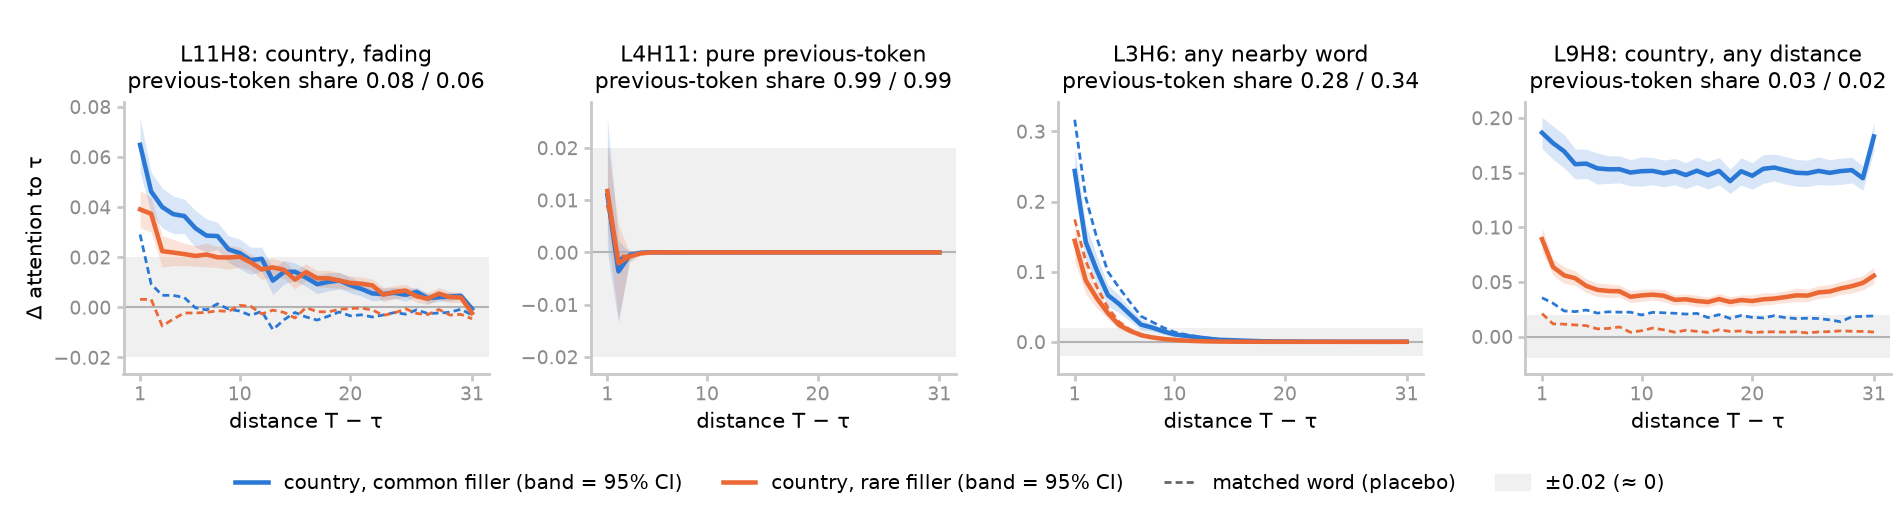
\includegraphics[width=\linewidth]{exp4_heads.png}\par}
{\small L11H8 looked like a previous-token head in Exp~10 only because its attention is otherwise diffuse, so an adjacent
country became its top key.\par}

\vspace{4pt}
\head{2 \textperiodcentered\ ``Previous-token'' heads react only nearby}{dots = BH $q \le 0.05$ and $|\Delta| \ge 0.02$}
{\centering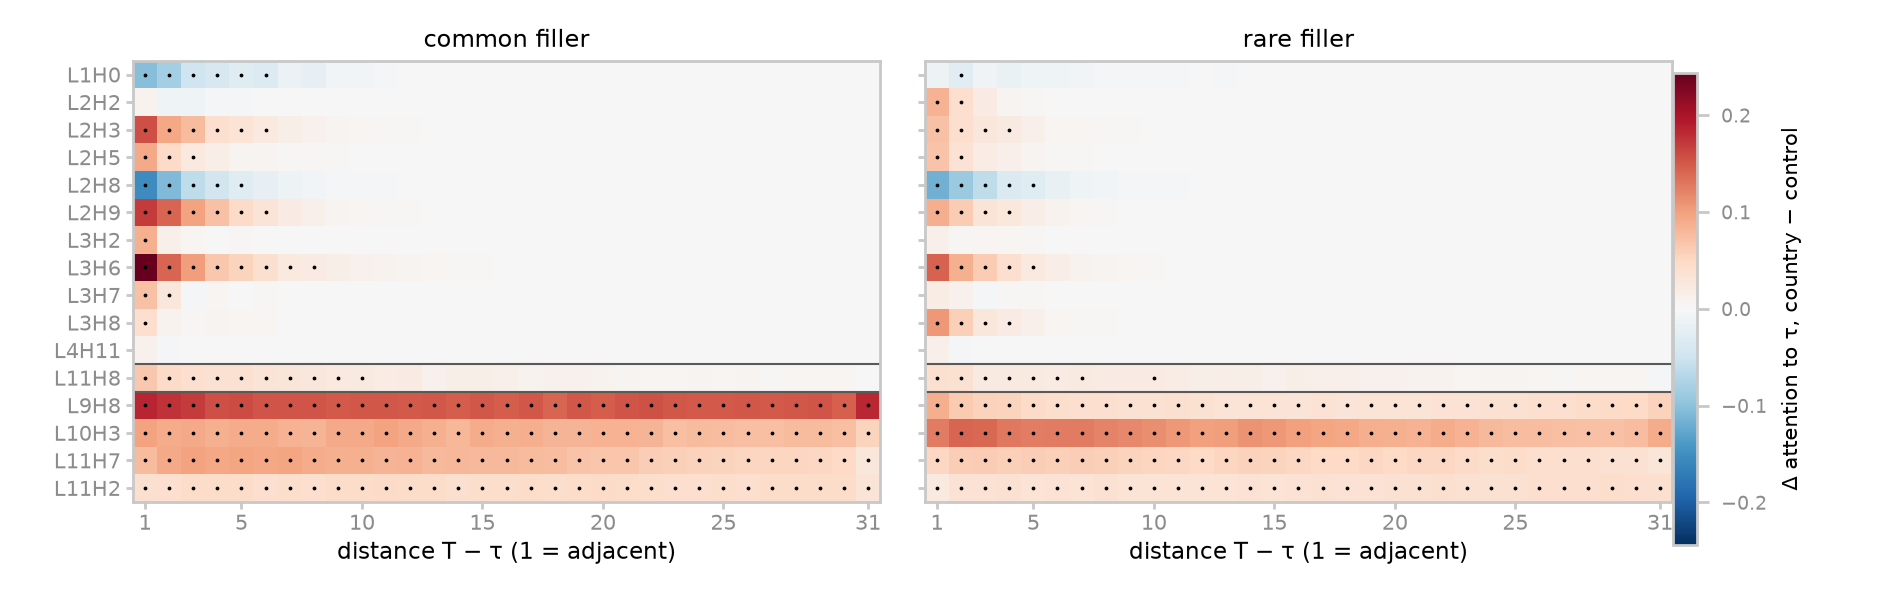
\includegraphics[width=0.8\linewidth]{exp4_grid.png}\par}
{\small Top: Exp~1's previous-token heads, nothing meaningful past distance 8. Middle: L11H8. Bottom: the four any-distance heads.\par}

\vspace{4pt}
\head{3 \textperiodcentered\ Depth and range (stretch)}{``layers 9--11 act globally'': only through four heads}
{\centering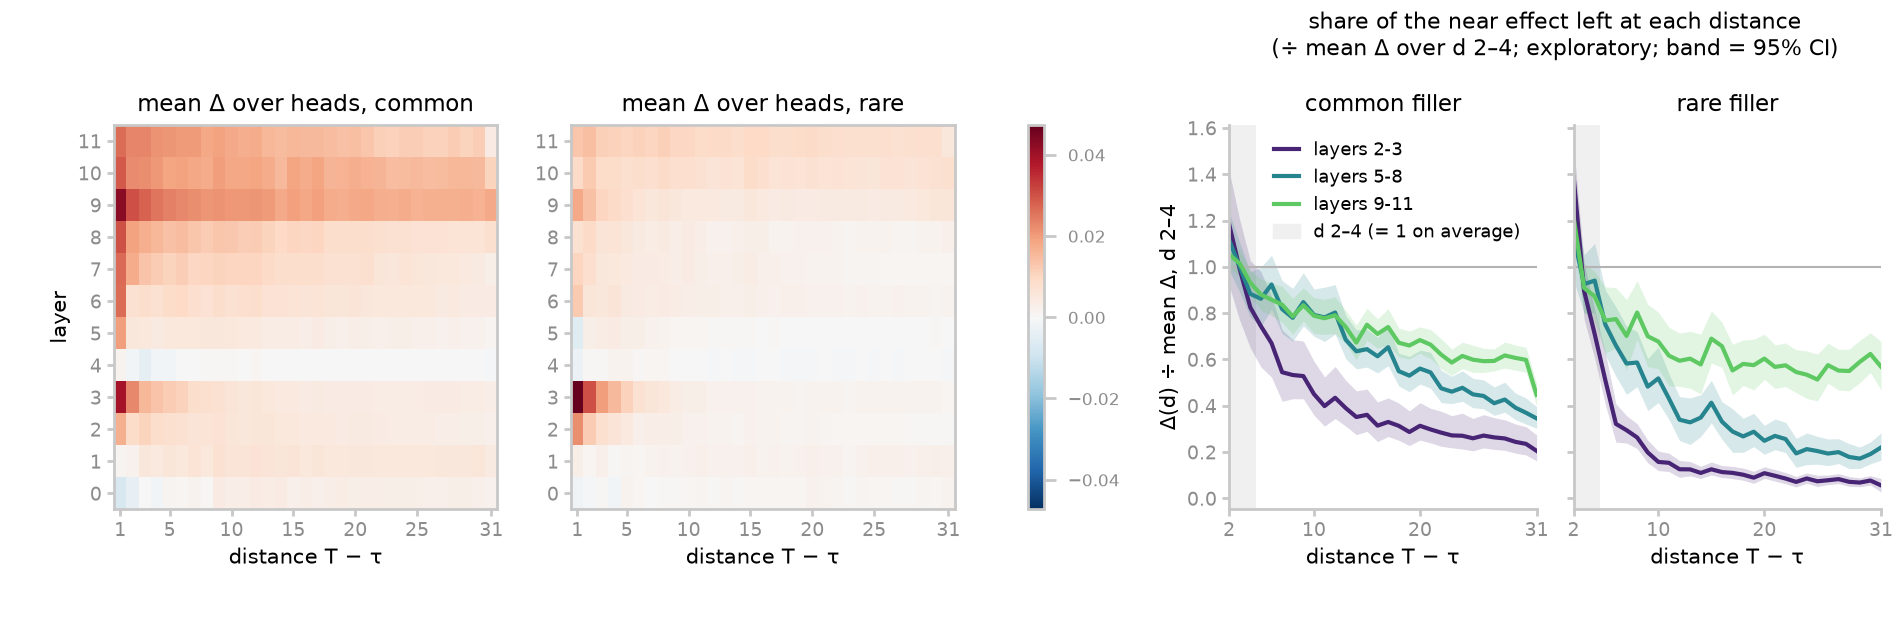
\includegraphics[width=0.8\linewidth]{exp4_layers.png}\par}
{\small Layers 2--3 act locally. Layers 9--11 keep about 60\% of their near effect past distance 16, but only because of the
four heads above. The pre-registered absolute test failed, because 9--11 are larger at every distance. The right panel is exploratory.\par}

\vfill
{\footnotesize\color{muted} Pre-registered (exp4/PREDICTIONS.md): C3--C6 pass. C1, C2 and H-loc fail. All checks pass, and an
independent Hugging Face recomputation matched to $6\times10^{-6}$. The placebo words are not frequency-matched, hence the probe.
Interactive: \href{https://pleyva2004.github.io/MechInterp/no-op-research/Experimen_1_Refactored/onepager/exp4_slider.html}{country slider},
\href{https://pleyva2004.github.io/MechInterp/no-op-research/Experimen_1_Refactored/onepager/exp4_viewer.html}{per-head viewer}.}
\end{document}
